\documentclass[12pt,oneside,openany,letterpaper]{article}


\usepackage{fancyhdr}
\usepackage{helvet}
\usepackage{amsmath}
%\usepackage{graphicx}
\usepackage{psfrag}
\usepackage{setspace}
%\usepackage[hypertex, linktocpage]{hyperref}[2003/11/30]
\usepackage[linktocpage]{hyperref}[2003/11/30]
\usepackage{lscape}
\usepackage{nicefrac}
\usepackage{mathrsfs}
\usepackage{units}
\usepackage{upgreek}
\usepackage{amssymb}
\usepackage{color}
\usepackage{wrapfig}
\usepackage{multirow}
\usepackage{url}
\usepackage{verbatim}
\usepackage[pdftex]{graphicx}
\usepackage{epstopdf}
\usepackage{enumitem}
\usepackage{wrapfig}
\usepackage{rotating}


\onehalfspacing \setlength\textheight{667pt}
\setlength\textwidth{506pt} \setlength\oddsidemargin{-18pt}
\setlength\topmargin{-20pt}
%\setlength\footskip{24pt}
\addtolength\headheight{2.5pt} \addtolength\headsep{-14pt}
%\fancyhead[R]{\includegraphics[height=10.5pt]{ubclogo_bw.eps}\#:  55907968}
%\renewcommand\familydefault{\sfdefault}


%\fancyhead[L]{Name:} \fancyhead[R]{Student
%Number:~~~~~~~~~~~~~~~~~~~~~~~~~~~~~~~~~~~~~~~~~~}
\fancyhead[L]{\emph{Introduction to Electronics}}\fancyhead[R]{ADC}
\fancyfoot[L]{PHYS 231}\fancyfoot[R]{Final Project}
\pagestyle{fancy} \pagenumbering{arabic}


\newenvironment{packed_enum}{
\begin{enumerate}
  \setlength{\itemsep}{0pt}
  \setlength{\parskip}{0pt}
  \setlength{\parsep}{0pt}
}{\end{enumerate}}


\newenvironment{packed_item}{
\begin{itemize}
  \setlength{\itemsep}{0pt}
  \setlength{\parskip}{0pt}
  \setlength{\parsep}{0pt}
}{\end{itemize}}


\begin{document}

\thispagestyle{plain}
\begin{center}
{\large{\bf{\fontfamily{phv}\selectfont Physics 231 - Analog-to-Digital Converter (Final Project)}}}
\end{center}

\noindent {\bf As preparation for the laboratory, examine the final circuit diagram at the end of these notes and write a brief plan for the project, including a list of the components needed and a layout of how the circuit will actually be assembled on your circuit board.  Complete this planning phase before coming to the lab.}

~

\noindent In this experiment you will construct an analog-to-digital converter (ADC), making use of several of the principles that we've studied in this course.  The ADC is a substantially larger and more complex circuit than the other circuits that we've studied in the PHYS~231 lab so far.  Our plan of attack will be to first build functional ``sub-circuits'' the perform specific tasks.  We'll then combine the sub-circuits together at the end to complete the analog-to-digital conversion.

~

\noindent SCHMITT-TRIGGER INVERTER

~

\noindent The MC54/74HC14A inverters (NOT gates) you have been using are a special type of inverter which incorporate hysteresis in the input triggering characteristic. In other words, the input
voltage level required to cause LO$\to$HI transitions is different than the voltage level required to cause HI$\to$LO transitions. This characteristic is shown graphically in Fig.~\ref{fig:schmitt}.

\begin{figure}[ht]
\centering
    (a)~\includegraphics[width=0.4\textwidth]{figures/stdNot.pdf}\qquad (b)~\includegraphics[width=0.4\textwidth]{figures/hystNot.pdf}
    \caption{Plot of $v_\mathrm{out}$ as a function of $v_\mathrm{in}$ for (a) a standard inverter and (b) an inverter with hysteresis.}
    \label{fig:schmitt}
\end{figure}

\noindent The presence of hysteresis of this kind increases the versatility of the unit. In particular, Schmitt-trigger circuits provide excellent noise immunity and the ability to ``square up''
signals with long rise and fall times. An application of interest to us is the ability to construct a simple ``square wave oscillator'' from such an inverter.

~

\noindent SQUARE WAVE OSCILLATOR

~

\noindent Assemble the circuit shown in Fig.~\ref{fig:SqWave}.
\begin{figure}[h!]
\centering
    
\includegraphics[width=0.375\textwidth]{figures/SqWave.pdf}
    \caption{A square wave oscillator made from an inverter with hysteresis.  Note that this circuit does NOT have an input.  All you need to do is power the IC with $+5\rm\ V$ and then monitor the output using the oscilloscope.}
    \label{fig:SqWave}
\end{figure}

\noindent For your ADC, you will need a ``pulse'' generator providing a stream of narrow pulses. These pulse will ultimately be used reset the ADC circuit such that it can track changes to the analog
signal at the input and update the final digital output.

~

\noindent PULSE GENERATOR

~

\noindent To generate the narrow pulses, connect the circuit shown in Fig.~\ref{fig:pulse} to the output of the square wave generator you just assembled (Fig.~\ref{fig:SqWave}).
\begin{figure}[h!]
\centering
    
\includegraphics[width=0.55\textwidth]{figures/pulse.pdf}
    \caption{When added to the output of the square wave oscillator, this circuit produces a stream of narrow pulses.}
    \label{fig:pulse}
\end{figure}

\noindent Now decrease the oscillation frequency of your square wave oscillator (Fig.~\ref{fig:SqWave}) by connecting a $220\rm\ \mu F$ capacitor in parallel with the existing $1\rm\ \mu F$ capacitor. 

\begin{quote}
{\bf Note}: Capacitors with large values of capacitance ($100$'s of $\rm \mu F$) are called electrolytic capacitors and they are {\it polarized} (i.e.\ they have negative and positive terminals).  The longer of the two leads is the positive terminal. The negative terminal is also marked by a black or grey stripe along the length of the cylindrical body of the capacitor.
\end{quote}

\noindent {\bf Leave this combination of circuits assembled on your breadboard.}  They will be incorporated into your final ADC circuit. See the sub-circuit labeled ``Reset Pulse Generator'' and enclosed by the blue box in Fig.~\ref{fig:ADC}.  At this point, you should use a piece of masking tape to label your breadboard with your name name and your partner's name.

~

\noindent CLOCK SIGNAL

~

\noindent For your ADC, you will require another square wave oscillator, a unit generating a
train of ``clock'' pulses which will then be ``counted'' by a counter IC.  Assemble the circuit shown in Fig.~\ref{fig:clock} on your breadboard.  Note that each inverter chip has six individual NOT gates.  Therefore, you can use the same chip used for the pulse generator when assembling the clock signal generator.

\begin{figure}[h!]
\centering
    
\includegraphics[width=0.6\textwidth]{figures/clockSignal.pdf}
    \caption{When added to the output of the square wave oscillator, this circuit produces a stream of narrow pulses.}
    \label{fig:clock}
\end{figure}

\noindent Assemble this circuit and make sure that it produces a square wave with a frequency of approximately $10\rm\ kHz$. The $10\rm\ k\Omega$ ``variable'' resistor allows you to tune the frequency of your
oscillator.

~

\noindent {\bf Leave this circuit assembled on your breadboard.}  It will be incorporated into your final ADC circuit. See the sub-circuit labeled ``Clock Generator'' and enclosed by the red box in Fig.~\ref{fig:ADC}.  

~

\noindent $\div 100$ COUNTER

~

\noindent Figure~\ref{fig:counter} shows how a 74HC390 counter chip can be used to assemble a ``$\div 100$'' counter.  The chip is equipped with two $\div 2$ counters and two $\div 5$ counters.  The combination of one $\div 2$ and one $\div 5$ counter results in the $\div 10$ counter.  The combination of the two composite $\div 10$ counters results in the desired $\div 100$ counter. It is convenient to use light-emitting diodes (LEDs) to monitor the digital output.  The $200\rm\ Omega$ resistors are to limit the current through the LEDs.

\begin{figure}[h!]
\centering
    \includegraphics[width=\textwidth]{figures/divideBY100.pdf}
    \caption{A $\div 100$ counter made from a 74HC390 counter IC.  LEDs are used to monitor the binary outputs.}
    \label{fig:clock}
\end{figure}

\noindent The positive terminals of the diodes should be connected to the counter outputs and the resistors should placed between the negative terminals of the LEDs and ground. Verify the operation of this whole counting system by feeding the TTL output of the function generator into the $\div 100$ counter clock input.  Use a low frequency so that you can easily resolve each state of the output. The counter should count from $0$ to $99$ and then return back to zero.

~

\noindent The $\div 10$ counters are equipped with a ``reset'' function. In normal operation, the reset inputs are grounded. Taking the reset input from LO$\to$HI$\to$LO resets the counters such that all outputs read LO. {\bf Keep this circuit assembled on your circuit board.} See the sub-circuit labeled ``Two $\div 10$ Counters \& Digital Output'' and enclosed by the purple box in Fig.~\ref{fig:ADC}

\clearpage

ANALOG-TO-DIGITAL CONVERTER

~

\noindent Even today, there is still a large body of instrumentation involving analogue signals (voltages and currents). In order to use a computer for monitoring, acquiring or processing data from such instrumentation, the analog information must first be converted to digital quantities. The ADC accomplishes this task.

~

\noindent There are many techniques utilized by commercial ADC's to perform the A-to-D conversion. One of the simplest methods (and still encountered in practice) involves an analog-to-time converter. This is a device which, on receipt of an appropriate ``trigger'' pulse, generates a ``stop'' pulse at a time $t$ later, where $t$ is proportional to the analog input voltage which is to be converted to a digital output.

~

\noindent By gating a free-running ``clock'' with a pulse whose time duration is equal to $t$, and counting the gated clock pulses in an appropriate counter, the desired analog-to-digital conversion is obtained. This is the type of ADC which you will assemble in this lab.

~

\noindent ANALOG-TO-TIME CONVERTER

~

\noindent We now develop the required analog-to-time conversion. As shown in Fig.~\ref{fig:ADC}, the circuit consists of two parts:
\begin{itemize}
\item The first part is a circuit which, on receipt of a ``start'' pulse (produced by the Reset Pulse Generator circuit), generates a ``ramp voltage'' (a linearly-increasing voltage signal).
\item The second is a voltage comparator which compares the input analog voltage, whose value is to be digitized, with this ramp voltage ramp, generating an output pulse, the ``stop'' signal, when the ramp exceeds the input.
\end{itemize} 

\noindent As well as resetting the ramp generator back to it quiescent (on inactive) state, this ``stop'' pulse also resets the flip-flop, thus stopping the clock pulses from reaching the $\div 100$ counter.

\clearpage

\begin{figure}[h!]
\centering
    \includegraphics[width=\textwidth]{figures/ATC.pdf}
    \caption{A ramp generator (integrator circuit) and comparator are used to accomplish the required analog-to-time conversion.  In Fig.~\ref{fig:ADC}, the ramp generator is labeled ``Integrator'' and is enclosed in a yellow box and the comparator is labeled ``DC Input \& Comparator'' and is enclosed in a red box.}
    \label{fig:ATC}
\end{figure}

\noindent In detail, the analog-to-time converter:
\begin{itemize}
\item The voltage ramp circuit is an op-amp integrator. Its input is a constant voltage of $-15\rm\ V$, which when integrated results in a positive ramp voltage at the output. The transistor in parallel with the feedback capacitor is an electronic switch controlled by the trigger input (a digital LO or HI).  When ``open'' (resulting when the trigger input is LO), the integrator operates in the fashion described above, producing the required ramp voltage at its output. However, when the switch is ``closed'' (resulting when the trigger input is HI), the feedback capacitor is short circuited such that $v_\mathrm{out} = v_-$.  However, since $v_+ = v_- = 0$, the output of the integrator circuit is zero in this case.
\item The LM311 comparator yields a HI or LO voltage level depending on whether the value of the ramp voltage is less than or greater than the input voltage set by the variable resistor. Operationally, as the ramp voltage moves past the input voltage level, the output of the comparator makes an abrupt HI$\to$LO transition.
\end{itemize}

~

\noindent Construct the ramp generator (with transistor switch) and comparator circuits using the LM741 op-amp, 2N3904 NPN transistor and LM311 comparator. Refer to the pin diagrams shown in the data sheets when assembling your circuits. Note that the pin assignments are different for the LM741 op-amp and the LM311 comparator!  {\bf Also note that, to function properly, pin 1 of the LM311 comparator must be connected to ground.}

~

\noindent To test the circuit, adjust the variable resistor so that a DC input voltage between zero and $+15\rm\ V$ is provided to the 311, and apply a square wave (HI$\to$LO$\to$HI) to the input of the transistor switch (labeled ``trigger input'' in Fig.~\ref{fig:ATC}). The TTL output of the function generator can be to supply the required square wave.  The period of the square wave should be long enough for the value
of the ramp to exceed the input dc signal level before the next LO$\to$HI transition at trigger input occurs. If this is not the case, decrease the frequency of the square wave (so as to increase its period).  At the instant the ramp voltage exceeds the DC signal level ($V_\mathrm{DC}$ in Fig.~\ref{fig:ATC}), the output of the comparator will transition from HI to LO. It switches back to HI when the ramp is turned off, which occurs when the trigger input returns to HI.

~

\noindent {\bf Caution}: Do not proceed further until you are sure that the output of the comparator varies between the HI and LO logic levels as described above. If you fail to follow this advice and proceed to the next section with an improperly functioning comparator, you may destroy some of the logic gates which will be connected to it!

~

\noindent ANALOG-TO-DIGITAL CONVERTER

~

\noindent You are now ready for the most exciting part of this project!

~

\noindent Assemble the complete ADC circuit shown in Fig.~\ref{fig:ADC}.  You will need to insert two more inverters, one NAND gate and assemble a flip-flop from two additional NAND gates.  Note that the additional inverters can come from the same IC you're already using.  All three NANDs can also be supplied from a single IC.  Connect your various sub-circuits together according to Fig.~\ref{fig:ADC}.  Carefully recheck that all required interconnections have been incorporated and then test your analog-to-digital conversion!

~

\noindent MODE OF OPERATION

~

\noindent The ``Reset Pulse Generator'' is the sub-circuit that determines the frequency at which your DC input $V_\mathrm{DC}$ is sampled. Its short (negative going) output is used to:
\begin{itemize}
\item Clear the decade counter. However, since the decade counter requires a positive reset (CLR) pulse, an additional inverter has been inserted between the Reset Pulse Generator and the CLR input of the counter.
\item ``Set'' the flip-flop which, in turn, opens a gate to allow clock pulses (from the ``Clock Generator'') to pass to the counter circuit. Since negative-going signals are required to ``set'' the flip-flop, the necessary signal could have been obtained directly at the output of the Reset Pulse Generator. However, in order to be certain that no gated clock pulses can arrive at the decade counter before the counter has been cleared, a slight time delay is intentionally introduced by using an additional inverter before the flip-flop. This inverter changes the short positive output pulse back to a short negative pulse.
\end{itemize}

\noindent In addition, the flip-flop opens the electronic (transistor) switch at the ramp generator to initiate the analogue-to-time conversion process.

~

\noindent Once the ramp voltage reaches the level set by the DC input $V_\mathrm{DC}$, the negative transition at the output of the LM311 comparator ``resets'' the flip-flop which, in turn, closes the gate at the output of the Clock Generator circuit, thus preventing any more clock pulses from reaching the counter.  The flip-flop reset also closes the electronic (transistor) switch which ``shorts'' the $1\rm\ \mu F$ capacitor in the feedback loop of the integrator.  When the switch closes, the ramp voltage is terminated and the output LM741 op-amp returned to ground. At this instant, the LM311 comparator responds by changing its output to HI. Since this whole process, which occurs after the ramp voltage reaches the level set by the $V_\mathrm{DC}$, takes such a short time, the duration of the negative output pulse from the comparator is extremely short in duration.

~

\noindent The whole cycle repeats when the next trigger pulse is received.

~

\noindent When your entire circuit appears to be behaving properly, measure the DC voltage $V_\mathrm{DC}$ and then vary the Clock Generator frequency by adjusting its $10\rm\ k\Omega$ variable resistor so that the counter displays the correct binary output. Specifically, calibrate your ADC such that a reading of 100 corresponds to an analog input of $V_\mathrm{DC} = 10.0\rm\ V$.

~

\noindent Finally, produce a timing diagram for the analog-to-digital converter by sketching in your lab notebook the shapes of the waveforms at various test points that illustrate how the different parts of the full circuit interact with one another.

~

\noindent If time permits, once your ADC is working properly, use two LTS-4301JR (or equivalent) seven-segment displays and two MC14495P1 (or equivalent) decoders to display your counter outputs as decimal numbers.  Look at pin diagrams on the data sheets archived on the course website to correctly wire the decoders and displays.

\begin{figure}[ht]
\centering
    \includegraphics[width=1.2\textwidth, angle=90]{figures/ADC.eps}%<---angle here
    \caption{The complete ADC circuit with the various sub-circuits highlighted.}
    \label{fig:ADC}
\end{figure}



\end{document}
